\chapter{序論}
\label{chap:intro}
\fancyhf{}
\rhead{\thepage}
\lhead{第\ref{chap:intro}章 序論}
\cfoot{\thepage}

本章では,本研究の背景,目的および本論文の構成について述べる.


\section{研究の背景}

\subsection{学習内容の個人最適化と学習科学}
% 導入:学習の個人最適化
近年,教育と情報技術の融合が進む中で,アダプティブラーニングという言葉が注目されている.
個人に最適化された学習内容の自動提供を実現するもので,その社会的影響の大きさからアメリカを中心として世界的に注目が集まっており,
関連するスタートアップや大学での研究に多額の資金が投入されている\cite{piccioli2014learning}.

学習内容を個人に最適化するという考え方は,決して新しいものではない.
現在の学校教育では,一人の教師が複数の生徒に対して同時に教育する形態が一般的であるが,
学習の速度や教科による得手不得手は人それぞれであり,
同じ教育を施しても,十分な理解ができずにつまずいてしまう生徒もいる.
そのような生徒に補習を行い,つまずきを克服する手助けをするような,
生徒の学習状態を考慮して教育を設計することは昔から行われてきており,
そうした指導が巧みな教師は「腕のいい」教師として評価されてきた.
しかし,こうした方法では,
習熟の遅い生徒を助けることに重きが置かれるため,習熟が周りより早い生徒への対応は後回しにされることが多く,発展的な学習機会や知的好奇心の向上を妨げることに加え,
現実的な時間と労力を考慮すると,全ての生徒に個別に対応することは困難である.

より個別に教育を受ける手段として,個別指導形式の塾や家庭教師,通信教育なども利用される.
生徒一人一人に教師がつくことで,生徒の習熟度合いを考慮して教育を設計でき,
また能力によって優先されたり後回しにされたりすることもないため,学習内容を個人に最適化するという目的の上ではより望ましい.
しかし,このように教育の粒度を細かくし,個人最適化を進めようとするほど,
教師一人あたりが担当できる生徒の数が減ることによる人材的・金銭的負担や,教師ごとの指導能力の違いなどの問題に直面する.
結局,このような教師のマンパワーに依存した方法では,
%すべての生徒に最適な学習内容を提供するという目的を達成するには障壁が残る.
誰もが平等に最適な教育を受けるという目的を達成するには障壁が残る.

すべての生徒に最適な学習内容を提供するには,
従来の教育学的な方式や知見だけでなく,
現代の情報技術を活用して,生徒の学習過程を分析し学習内容を決定するような,新たな教育システムが必要である.
このように,教育と情報技術の融合により,
理論だけでなく実効性のある新たな教育システムを作り上げようとする動向は「学習科学」という研究分野として確立され,今日大きな注目を集めている\cite{白水始2014学習科学の新展開}.


\subsection{オンライン教育サービスの普及と学習効果分析の発展}
% 背景1:オンライン学習サービスを利用した個人最適化,データ蓄積に伴う学習効果分析の進展
アダプティブラーニングを始めとする教育と情報技術の融合の躍進には,
オンライン教育サービスの普及が背景にある.
オンライン教育サービスとは,
学校の教室で一人の教師が複数の生徒に対して同時に授業を行う従来の教育形態と異なり,
PCやモバイル端末を通じて,
オンライン上で提供される学習コンテンツを生徒が個人で利用するサービスを指す.

オンライン教育サービスの一つであるMassive Open Online Courses(MOOCs)\cite{mcauley2010mooc, pappano2012year,siemens2013massive}は,
多様な分野や難易度の講義から,時間や場所を問わずに,生徒が自分のペースで学習したいものを選択して学習できるというもので,
生徒が自身の習熟度合いに沿った教育を受けられないという問題を解決するプラットフォームとして,活用が期待されている.
例えば,世界最大級のMOOCsの一つであるCoursera\footnote{\url{https://www.coursera.org/}}は,
2017年1月の時点で,
29の国にまたがる148の教育機関とパートナーシップを結び,
コンピュータサイエンス,数学や論理,社会科学などに関する1600以上の講座を,2200万人以上に提供している.
日本では2013年2月に東京大学がCourseraに,2013年5月に京都大学がedX\footnote{\url{https://www.edx.org/}}に参加を表明したことから普及し,
2013年11月には日本版のMOOCsとしてJMOOC\footnote{\url{https://www.jmooc.jp/}}が設立されるなど,
国内外でMOOCsの利用が拡大している.

多様な講座を多くの人に提供するMOOCs以外にも,
より個人の学習過程をサポートすることに特化して設計される
Intelligent Tutoring System(ITS)と呼ばれるオンライン自動学習支援システムの利用も拡大している.
世界最大級のITSであるKnewton\footnote{\url{https://www.knewton.com/}}では,
生徒の学力や理解度と,学ぶべき対象をマッピングすることで、
生徒に最適な学習過程を設計し,
かつ生徒の学習の進捗に応じてその過程を動的に変化させる仕組みを有している\cite{upbin2012knewton}.
近年ではITSとMOOCsの融合も進んでおり\cite{aleven2015beginning},
オンライン教育サービスの利用は世界中で拡大している.

%日本でも,生徒が自宅でオンライン教育サービスを用いて知識を学び,
%学校ではより参加型のディスカッションを行うという「反転学習」の試みが提唱されており,
%オンライン教育サービスが社会に与える影響は今後さらに大きくなっていくといえる\cite{lage2000inverting, 重田勝介2014反転授業}.


% 背景1−B:オンライン教育サービスによるビッグデータの蓄積と活用
さらに,オンライン教育サービスは,新たな学習形態を提供するのみにとどまらず,
これまで困難であった大規模な学習効果分析を可能にするプラットフォームとして期待されている.
オンライン教育サービスでは,
提供された講義を生徒が学習する際に,その学習行動ログをデータとして蓄積することが可能なため,
そうして蓄積された多様な学習者の大規模な学習行動ログから,多様な学習効果の分析が可能になった.
特に,演習問題の回答ログは,その問題が問う知識を学習者が獲得しているか否かを表すため,Knowledge Tracingと呼ばれる知識獲得の分析に利用できる\cite{corbett1994knowledge}.
例えば,生徒の問題回答ログを利用して知識獲得の予測を行った研究\cite{machardy2015toward}は,
世界的に有名なMOOCsの一つであるKhan Academy\footnote{\url{https://www.khanacademy.org/}}に蓄積された100万件以上の問題回答ログを使用しており,
教育の分野における大規模な学習効果分析の一つである.
生徒が個人で利用するというオンライン教育サービスならではの特性によって,
このような研究成果を元に最適化された学習コンテンツを,個人に提供することが容易になったため,
教育の個人最適化に関する研究は,急速に活発化している.


\subsection{深層学習の躍進と知識獲得予測}
% 背景2:深層学習の高まり
一方,近年,教育に限らない多くの研究領域で,深層学習が注目されている.
深層学習とは,人間の脳の神経回路を模した多層のニューラルネットワーク構造を用いる機械学習の一分野で,
従来の機械学習では,人間が問題の特徴を捉えて素性を設計する必要があったが,
深層学習では,目的に応じた素性を,データから自動で学習することが可能になり,
画像認識\cite{schroff2015facenet,szegedy2014going},
音声認識\cite{hinton2012deep, bahdanau2015end},
機械翻訳\cite{sutskever2014sequence, dong2015multi}等,
多様な研究領域で飛躍的な進展が報告がされている.
直近の一年間では,
画像から動画を生成する研究\cite{vondrick2016generating}や,
会話を人間と同程度に認識できるとする音声認識の研究\cite{xiong2016achieving},
一部の欧米言語間の文レベルで,ほぼ人間と同等に正確な翻訳を実現したとする機械翻訳の研究\cite{wu2016google}なども報告されており,
深層学習によって,日々驚異的な成果が生み出されている.
また,2016年3月に人間のプロを倒したことで一躍有名になった,Google Deep Mindが開発したコンピュータ囲碁プログラムの「AlphaGo」\cite{silver2016mastering}は,
過去の人間の対局の記録である棋譜から,深層学習によって人間の囲碁の打ち方を学習し,自己対局による強化学習を通して,
今後10年は不可能と言われていた,人間のプロを打ち負かすほどの棋力を獲得した.
AlphaGoは,単に人間の打ち方を真似ただけでなく,
それまで人間が考えつかなかったような斬新な手を学習しており,囲碁界に衝撃を与えている.
このように,深層学習は,人間が認識できないようなデータの複雑な特徴を捉えることで,
これまで人間が作り上げてきた概念を大きく塗り替える可能性を秘めている.


こうした深層学習の技術は学習効果の分析にも活用が期待されており,中でも深層学習の適用によって大きく進展した分野として,知識獲得予測の研究が挙げられる.
知識獲得予測とは,生徒が特定の知識を獲得しているか否かを予測するタスクのことで,
生徒の学習行動をモデリングして各生徒の知識ごとの習熟度合いを正しく把握することにより,
よりレベルの高い問題に着手する前に必要な知識を確実に習得できるようにカリキュラムを設計したり,
生徒の苦手な部分に特化して学習サポートを行うなど,
生徒の学習効率を最大化することを目的とした研究である.

知識獲得予測の研究自体は以前から存在し,
知識獲得の時系列性に着目する系統と,知識間の関係性に着目する系統という2つのアプローチが存在したが,
このような伝統的なアプローチは,どれも知識獲得の時系列性か知識間の関係性のどちらかに傾倒してしまい,
知識獲得を包括的にモデリングすることができていなかった.
そのような系譜の中,\cite{piech2015deep}らが発表した,知識獲得予測に深層学習を活用するDeep Knowledge Tracing(以下,DKT)という手法では,
時系列分析でよく用いられる深層学習モデルであるRecurrent Neural Networks\cite{williams1989learning}を活用することで,
知識獲得の時系列性と知識間の関係性の双方を考慮した知識獲得予測が行え,
高い性能で知識獲得を予測できる上,
予測モデルを分析することで知識間の関係性をネットワークとして抽出できることが報告された.

知識獲得予測は,分析対象となるデータが取得でき,その成果も提供できるという点でオンライン学習サービスと非常に相性がよいため,
オンライン教育サービスの普及に合わせ,
DKTのような深層学習を適用する最先端の手法を中心に,研究が活発化している.

\subsection{知識獲得予測の問題点}

しかし,このような知識獲得予測の最先端の手法においても,ある問題が存在する.
知識獲得を予測するアルゴリズムの部分には深層学習を適用しているものの,
獲得の対象とされる「知識」は事前に人間が作成した知識分類によって定義され,所与のものとされている.
人間が作成した知識分類は,伝統的な枠組みや可読性といった定性的な尺度で作成されたものが多く,
実際の生徒の知識獲得の予測という定量的な文脈において最適に構造化されているという根拠はないため,
それを用いた知識獲得予測自体も最適なものとはいえない.

例えば,日本の学校教育では,基本的に
文部科学省が定めた学習指導要領\cite{gakushushidouyouryou}に基づいて教育カリキュラムが設計されており,
この学習指導要領が,生徒が学ぶ学問体系を構造化する知識分類の代表例といえる.
しかし,この学習指導要領は,一部の教育現場で実験が行われたり,時代に沿った教育内容の見直しはされているものの,
その根底にある理念は「全国のどの地域で教育を受けても、一定の水準の教育を受けられるようにするため」\cite{gakushushidouyouryou}というものである.
そのため,国全体としての教育の方向性を決定づけ,一定の教育水準を保つ目的においては有効なものの,
実際の生徒の知識状態を把握し,知識獲得を予測する上で最適に構造化された分類であるとはいえない.


また,近年のオンライン教育サービスの普及に伴い,
プログラミングやビジネス,資格試験やヘルスケアなどといった,これまでの伝統的な学問体系の範疇を超えた新たな学問が続々と登場している.
生活や職業が多様化した世相に合わせて,こうした新たな学問は誕生するものの,
学問としての歴史が浅く,その学問を司る正統な機構も存在しないことが多いため,体系が構造化されていない場合が多い.
例えば,図\ref{fig:business}はJMOOCにおけるビジネス教育の講座の一例だが,多様な機関が思い思いに講座を提供するため,
多様な講座を受講できるというメリットの一方で,学習コンテンツが構造化されずに雑多に広がる状況を生み出している.

\begin{figure}[htb]
\begin{center}
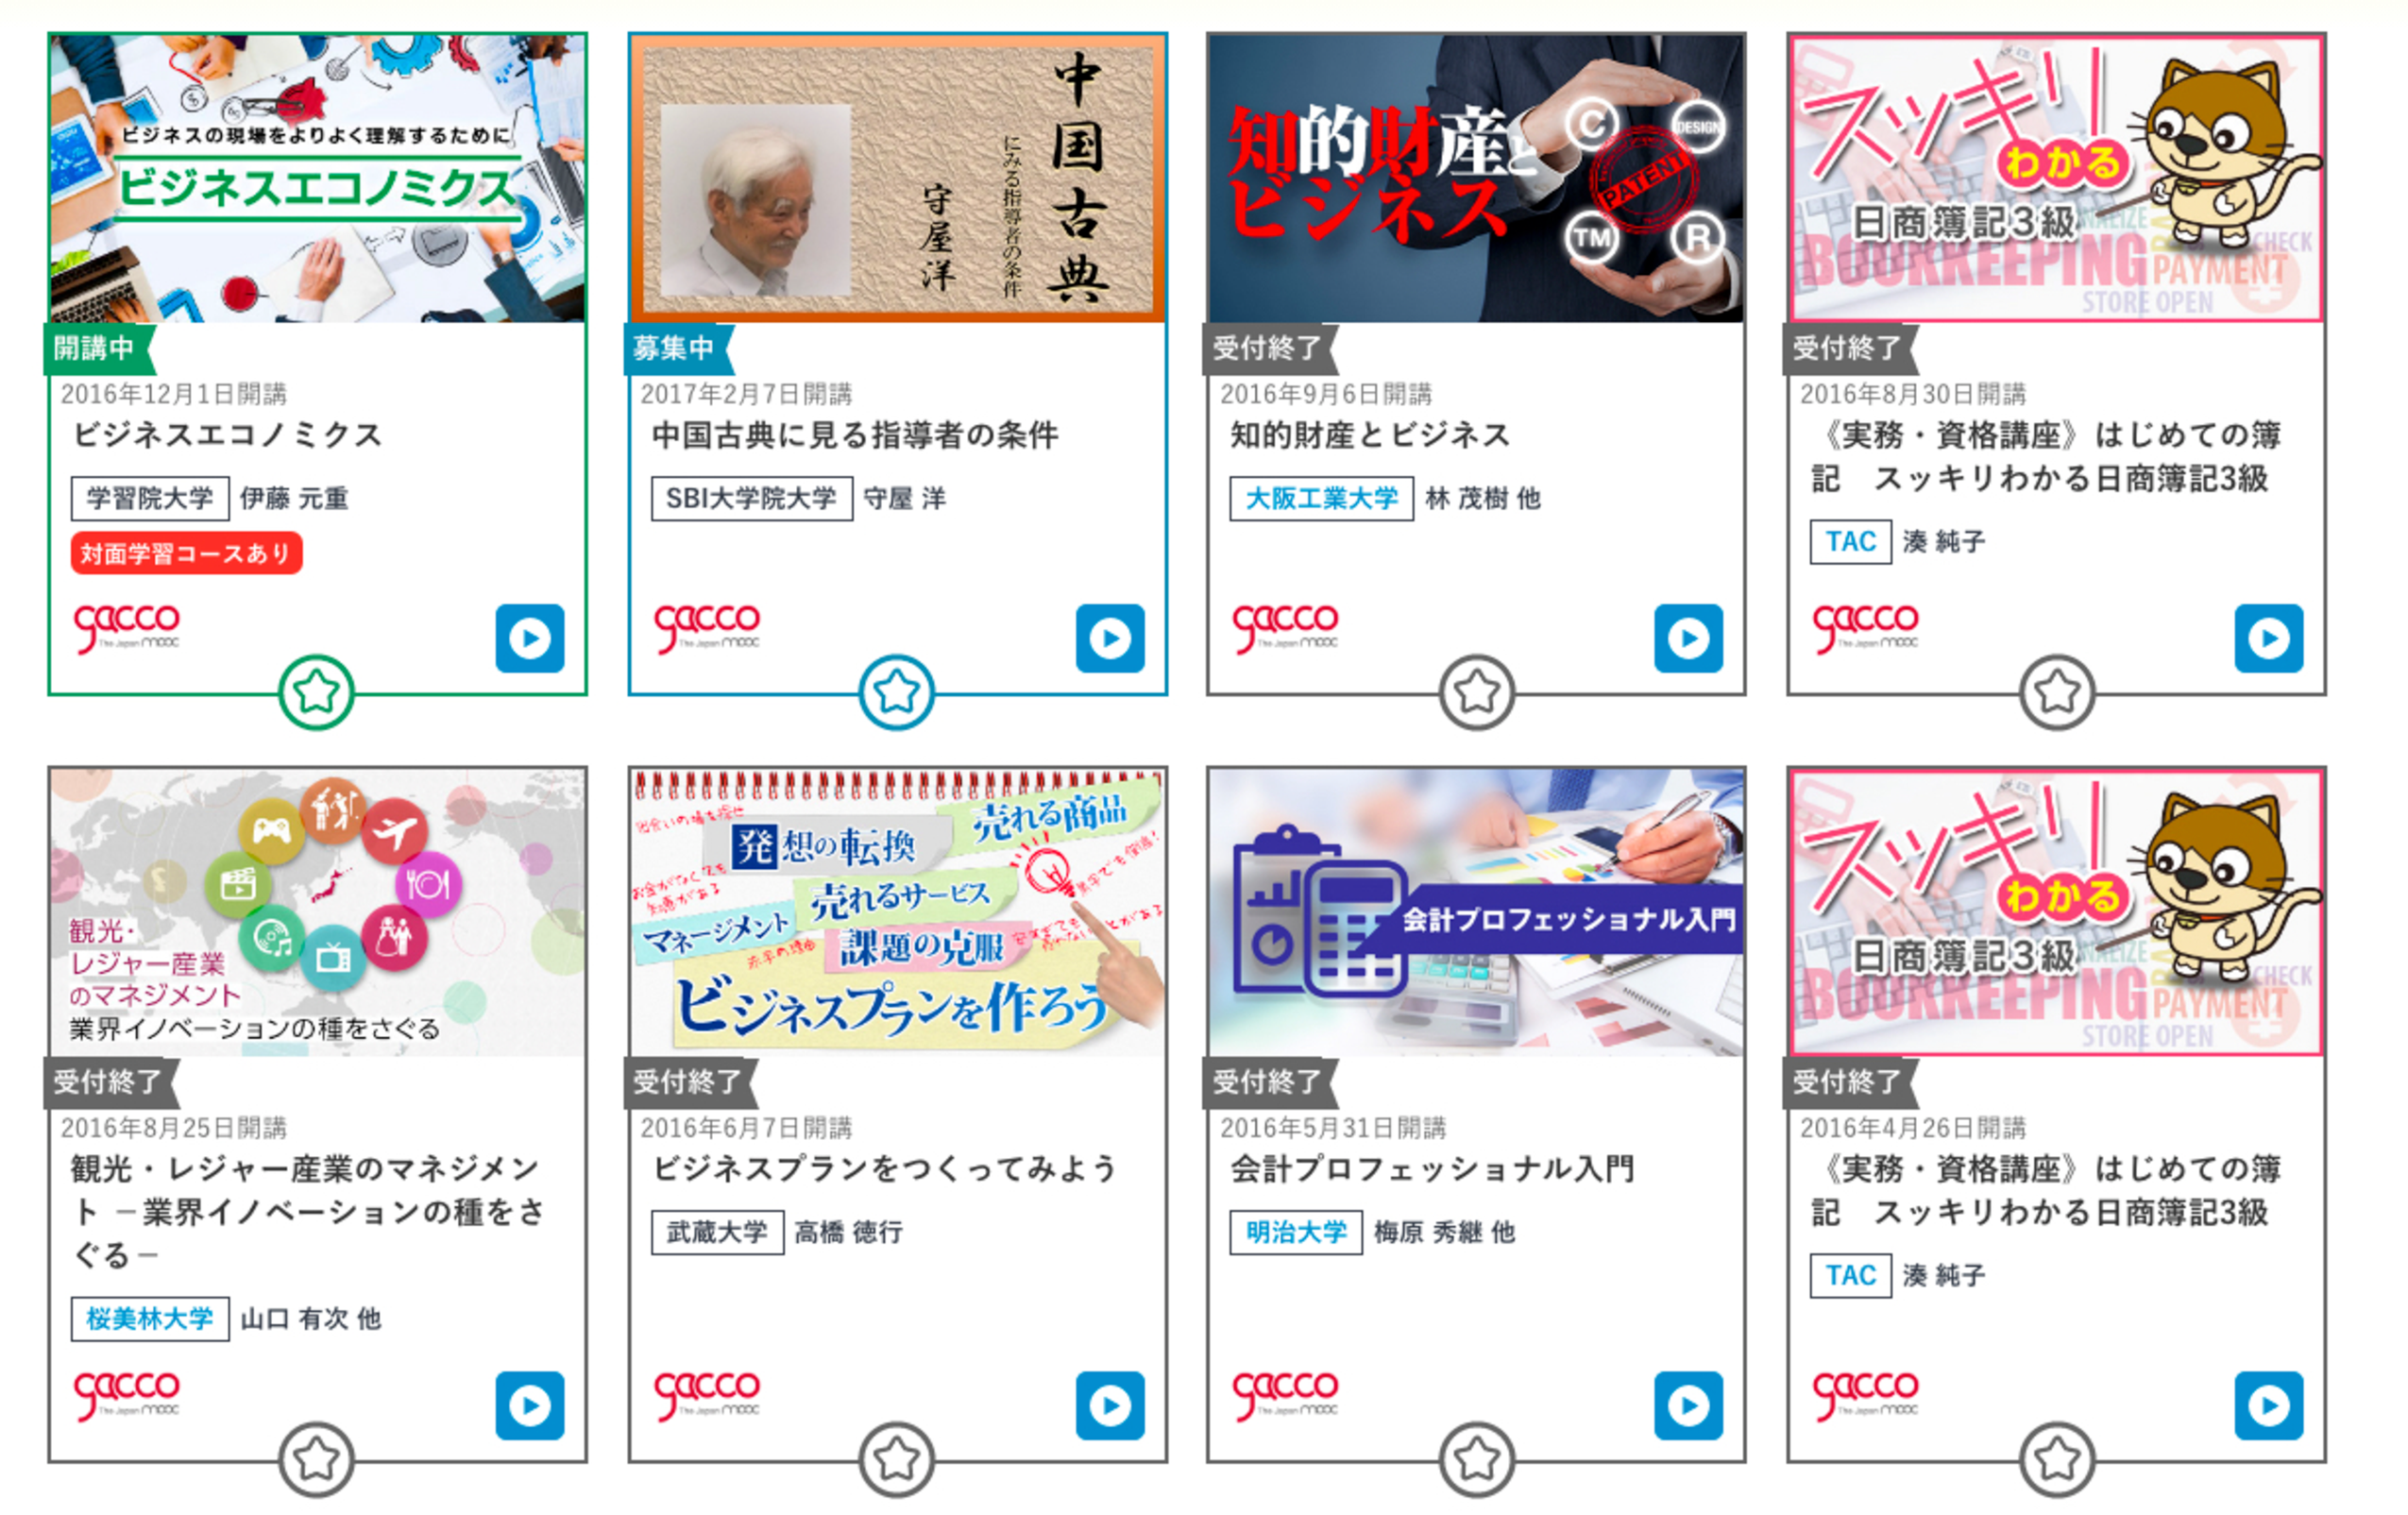
\includegraphics[width=400pt]{./img/business.pdf}
\end{center}
\caption{JMOOCにおける「ビジネスと経営」講座の一例}
\label{fig:business}
\end{figure}


学問体系を最適に構造化することは,学習者にとっても,指導者にとっても価値が高い.
学習者にとっては,学問体系が最適に構造化されるように知識が分類されることで,
より効率の良い順序で知識を獲得していくことが可能になり,
また,自身への教材推薦や学習サポートなどの個人最適化の精度も向上することで,学習効率の向上につながる.
指導者にとっても,
適切に構造化された知識分類を元に,既存の教材やカリキュラムを再検証したり,より生徒の習熟に効果的な教材を考える事が可能になる.
結果的に,学ぶ側と教える側の双方によって学問の質が高められることにより,その学問自体の発展にも寄与するといえる.

このように,
定量的な根拠に基づいて構造化されていなかったり,そもそも構造化されていない学問体系に対して,
知識獲得の予測性を最適化するように構造化して知識分類を作成することは,学術的にも,実用的にも価値が高い.
%人間が作成した知識分類というのは,
%「知識の体系はこうなっているはずだ」ないしは「この体系に基づいて教える・教えられることが望ましい」という専門家の仮説や理論に基づいて作られたものである.
今日多様な分野で成果を生んでいる,データから特徴を自動で学習できる深層学習を活用すれば,
人間が認識できないような,人間の知識獲得の複雑な過程を反映した,知識獲得予測を最適化するような構造を持った知識分類を学習できる可能性は高く,
生徒の学習効率を最適化するという最終的な目標を真に達成するには,
知識分類自体も深層学習によって最適化される必要があるといえる.



以上の問題意識に基づいた,既存研究と本研究の差分のイメージを図\ref{fig:problem}に示す.

\begin{figure}[htb]
\begin{center}
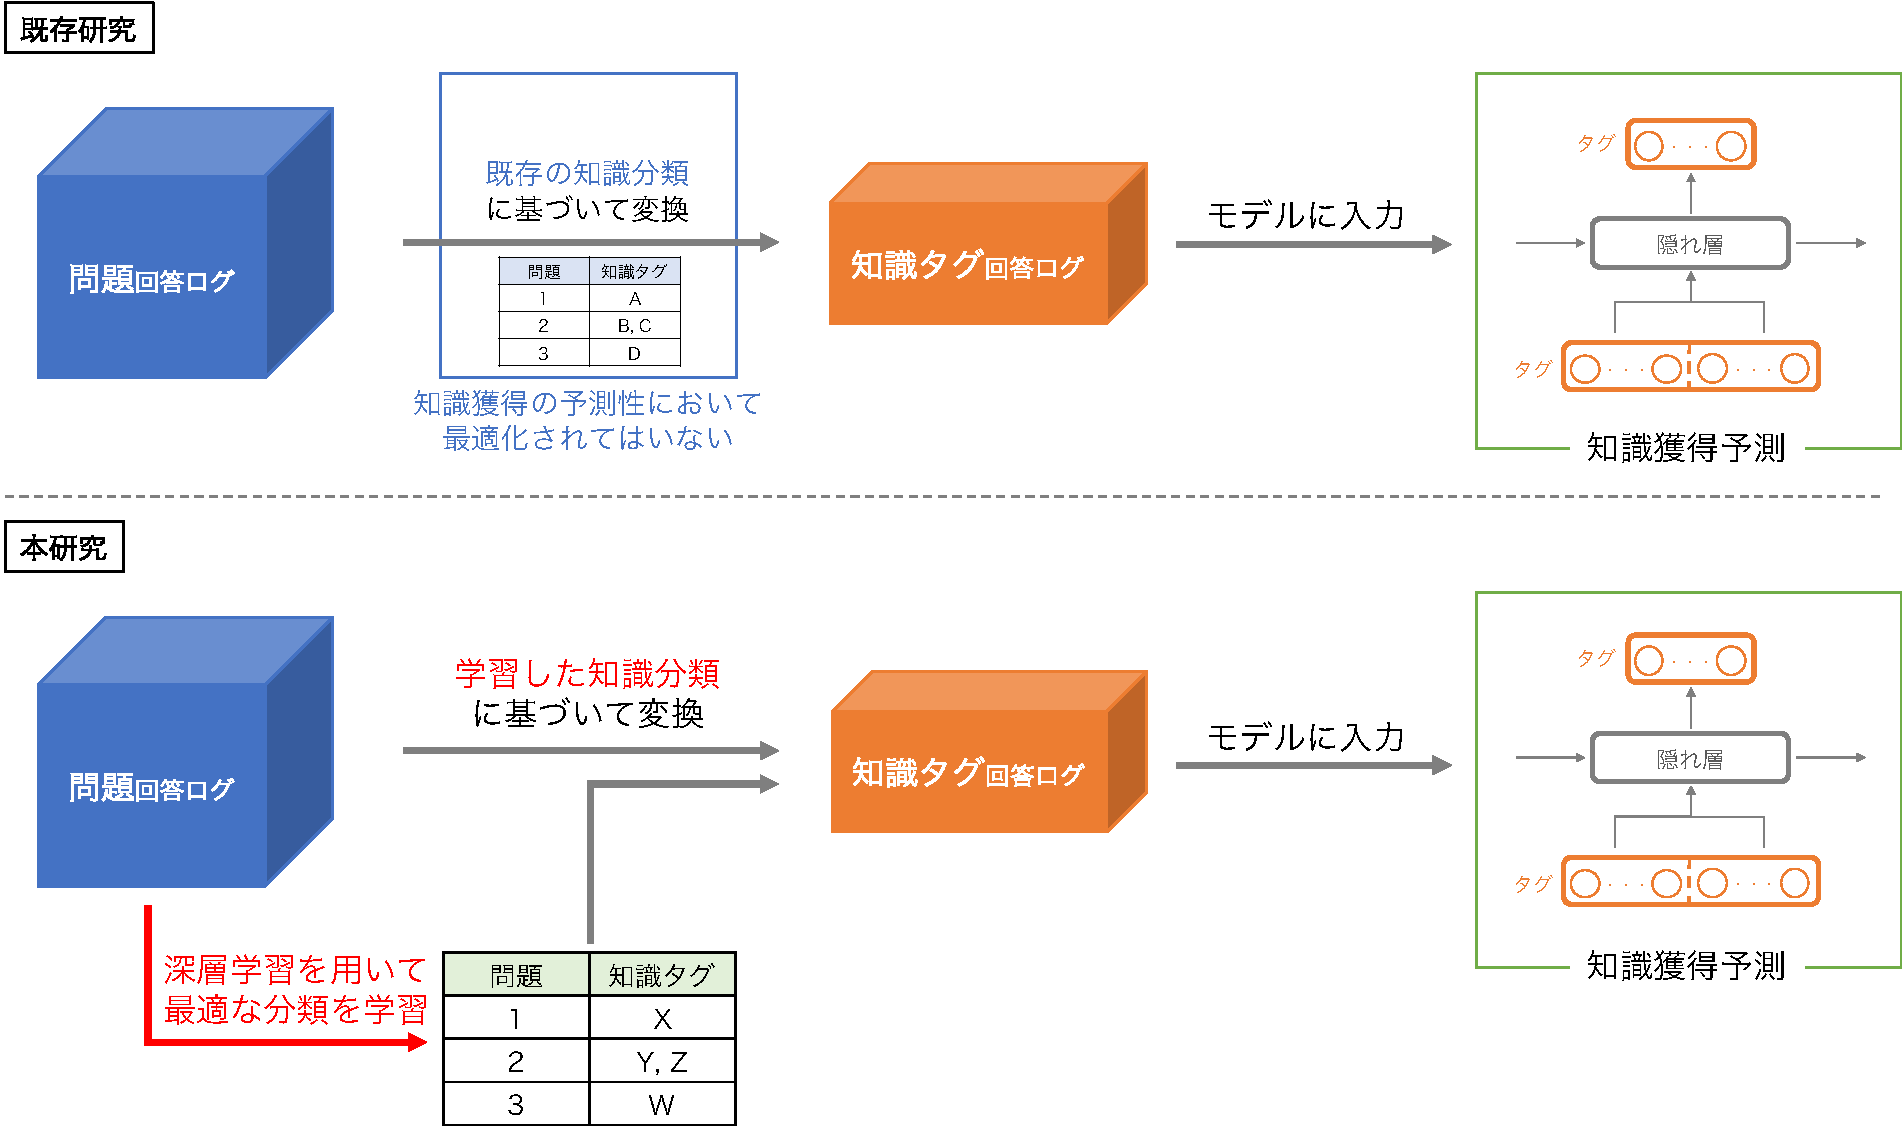
\includegraphics[width=400pt]{./img/problem3.pdf}
\end{center}
\caption{既存研究と本研究の差分のイメージ}
\label{fig:problem}
\end{figure}


\section{研究の目的}
本研究では,
現在の知識獲得予測に用いられている,人間が作成した知識分類は,知識獲得の予測を行う上では最適化された表現ではない,という仮定に立ち,
以下を検証することを目的とする.

\begin{itemize}
\item 深層学習によって抽出した知識分類を用いることで,人間が作成した知識分類を用いる場合よりも,高い精度で知識獲得予測を行うことができる.
\end{itemize}

本論文では,人間が作成した知識分類を所与のものとせずに,
問題の回答ログデータのみを深層学習に適用して知識獲得予測を行う過程で,
その予測性を最適化する知識分類を抽出することを目的としている.
従来,人間が事前に分類することが必要であった問題コンテンツの集合から,
知識獲得の予測性を最適化する知識分類を深層学習によって自動で抽出し,構造化できることを明らかにすることは,
生徒の学習効率の向上や学問体系の再構築・発展につながるだけでなく,
人間の学習や知識のメカニズムを解明することにもつながり,学術的な意義が大きいと考える.


\section{本論文の構成}
以降の本論文の構成について述べる.

\vvspace

第2章では,関連研究について述べる.
本研究と関連する既存の研究を俯瞰し,
周辺概念を整理することで,本研究の学術的位置づけを明確にする.

\vvspace

第3章では,提案手法について述べる.
まず,生徒の回答正誤を予測する過程で最適な知識分類を学習・抽出する手法について説明し,
また,抽出された知識分類を分析する手法について説明する.

\vvspace

第4章では,
実験で用いるデータセットについて述べる.
オンライン教育サービスにおける生徒の学習回答ログである,2つのデータセットを紹介し,
本研究に適用するための事前の処理を説明する.

\vvspace

第5章では,実験について述べる.
本研究で行う実験を大きく3つに分け,各実験の設定を述べた後,
実験結果について述べる.
実験結果においては,
提案手法によって抽出された知識分類を用いることで,既存の知識分類を用いた場合よりも高い精度で知識獲得を予測できることを示し,
予測性を最適化する構造を持つ知識分類が抽出されたことを定量的に確認する.
さらに,抽出された知識分類を既存の知識分類と定量的・定性的に比較することで,その性質を解釈する.

\vvspace

第6章では,実験結果を踏まえた考察を述べる.
まず,本研究で用いた手法の有効性や本手法によって得られた知識分類の性質を考察する.
また,
本研究で用いた手法の汎用性と実用性について考察し,
本手法が適用できるデータ範囲について述べ,
実際の教育現場への適用についても述べる.
さらに,
今後の展望として,
より良質な知識分類を得るためのモデルの改善や,
学習科学における対象データの拡大,
また,学習科学以外の分野への応用の可能性を考察し,本手法の一般性を述べる,

\vvspace

最後に,第7章で結論を述べる.
% もうちょい書く?
